\documentclass[11pt]{article}

\usepackage{graphicx}
\usepackage[top=25mm, bottom=25mm, left=25mm, right=25mm, a4paper]{geometry}
\usepackage{amsmath}
\usepackage{enumitem}
\usepackage{float}
\usepackage{fancyhdr}
\usepackage{booktabs}
\usepackage{tikz}
\usepackage{steinmetz}
\usepackage{pgfplots}

\pagestyle{fancy}
\fancyhf{}
\fancyhead[R]{Baturay Kafkas - 2240357068 - Electrical \& Electronics Engineering}

\rfoot{\thepage}
\renewcommand{\headrulewidth}{0pt} 
\renewcommand{\footrulewidth}{0pt}
\sloppy

\begin{document}

\begin{center}
\large
\textbf{ELE214 - Electronics Laboratory I Preliminary Work 4}
\end{center}

\section{Questions}

\begin{enumerate}[leftmargin=*,label=\textbf{\arabic*.}]

\item Explain the use of each circuit element in the figure briefly.

\begin{figure}[H]
    \centering
    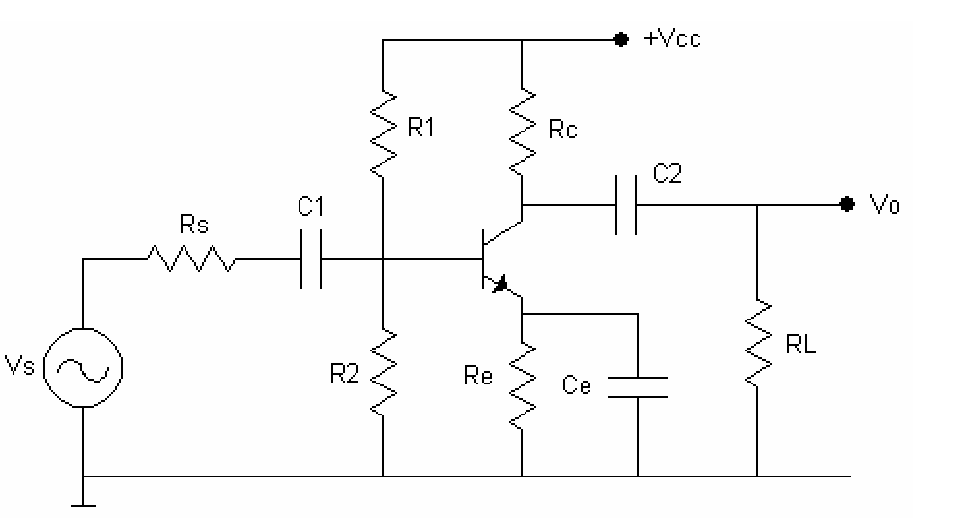
\includegraphics[width=0.75\linewidth]{Kt0o5zjbUB.png}
    
    \small \textit{Figure 1}
\end{figure}

\item Design an amplifier to produce a maximum swing with the following parameters: AC voltage gain: 50, $V_{CC}=15\text{ V},\:h_{fe}=100,\:V_{ce, \text{ sat}}=0.2\text{ V}$.
\end{enumerate}

\textbf{Experimental Work (Simulation of 1-4)}

\begin{enumerate}[leftmargin=*,label=\textbf{\arabic*.}]

\item Set up the circuit in \textit{Figure 1} with the following component values:
\[R_s=22\:\text{k}\Omega\qquad R_1=56\:\text{k}\Omega\qquad\ R_2=12\:\text{k}\Omega\]
\[R_3=R_c=3.3\:\text{k}\Omega\qquad R_e=1\:\text{k}\Omega\qquad\ R_L=2.2\:\text{k}\Omega\]
\[C_1=C_2=C_3=10\:\mu\text{F}\qquad V_{CC}=15\text{ V}\qquad V_s=1\:\text{kHz sinus}\]

\item Measure the $I_{C,Q}$ and $V_{CE,Q}$ of the circuit.

\item Taking $V_s=3V_{pp}$, obtain the transfer characteristics ($V_o$ vs $V_s$) on the oscilloscope. 

\item Taking $V_s=0.5V_{pp}$, measure $V_o$ with and without $R_L$. 

\end{enumerate}

\section{Answers}

\begin{enumerate}[leftmargin=*,label=\textbf{\arabic*.}]

\item $V_s$: The AC input signal to be amplified.

$R_s$: Source resistor.

$R_L$: Load resistor.

$R_c$: Collector resistor.

$R_e$: Emitter-degeneration resistor stabilizing the circuit.

$R_1, R_2$: Resistors that help the transistor work in the active region, or simply biasing.

$C_1, C_2$: Filter capacitors allowing AC input to pass and block DC input.

$C_e$: Emitter bypass capacitor increasing gain.

\item To achieve maximum symmetrical swing, the collector-emitter voltage $V_{CEQ}$ is centered:
\[V_{CEQ} = \frac{V_{CC} + V_{ce, \text{sat}}}{2} = \frac{15\text{V} + 0.2\text{ V}}{2} = 7.6\text{ V}\]

Assuming $I_{CQ} = 1\text{ mA}$, the thermal resistance $r'_e$ is:
\[r'_e = \frac{26\text{ mV}}{1\text{ mA}} = 26\:\Omega\]

The gain for the swamped amplifier is defined by:
\[A_v = \frac{R_C}{r'_e + R_{e1}} = 50\]

Setting $V_{R_C} = 6\text{ V}$ and $V_{R_E} = 1.4\text{ V}$,
\begin{itemize}
    \item $R_C = \dfrac{6\text{ V}}{1\text{ mA}} = 6\:\text{k}\Omega$,
    \item $R_{e1} = \dfrac{R_C}{A_v} - r'_e = \dfrac{6000}{50} - 26 = 94\:\Omega$,
    \item $R_{e2} = \dfrac{1.4\text{ V}}{1\text{ mA}} - 94\:\Omega = 1306\:\Omega$.
\end{itemize}

With $V_B = V_{R_E} + V_{BE} = 2.1\text{ V}$ and $I_{div} = 10 \cdot I_B$,
\[R_2 = \frac{2.1\text{ V}}{100\:\mu\text{A}} = 21\text{ k}\Omega, \quad R_1 = \frac{15\text{ V} - 2.1\text{ V}}{110\:\mu\text{A}} = 117.3\text{ k}\Omega\]

\begin{figure}[H]
    \centering
    
\includegraphics[width=0.55\linewidth]{q2.png}
\end{figure}
\end{enumerate}

\newpage

\textbf{Simulation}

\begin{enumerate}[leftmargin=*,label=\textbf{\arabic*.}]

\item The circuit with the indicated components:

\vspace{-2em}

\begin{figure}[H]
    \centering
    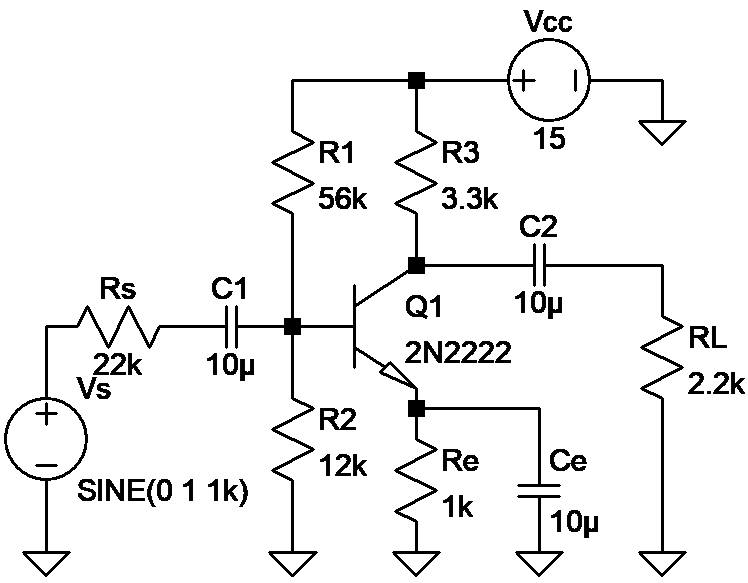
\includegraphics[width=0.55\linewidth]{e_q1.png}

    \small \textit{Circuit 1}
\end{figure}

\item Obtain the DC-equivalent circuit. $V_{CE,Q}\approx 6.91\text{ V}$ and $I_{CE,Q}\approx1.88\text{ mA}$.

\begin{minipage}{0.57\textwidth}
\begin{figure}[H]
    \centering
    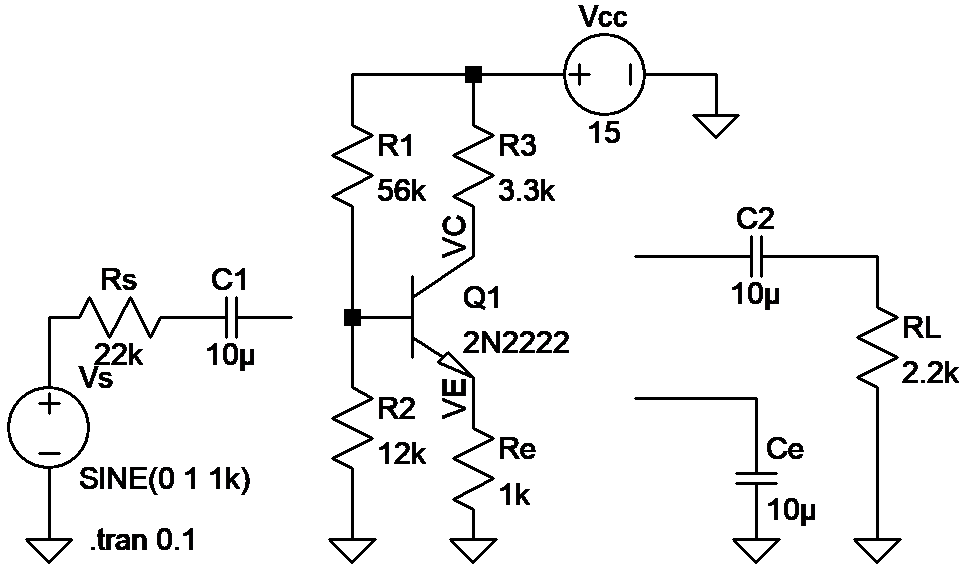
\includegraphics[width=1\linewidth]{e_q2.png}
    
    \small \textit{Circuit 2}
\end{figure}
\end{minipage}\hfill\begin{minipage}{0.43\textwidth}
\begin{figure}[H]
    \centering
    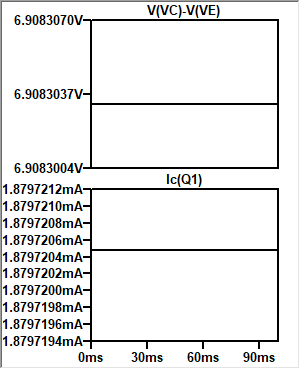
\includegraphics[width=0.75\linewidth]{LTspice_YTdLrSASik.png}
    
    \small \textit{Graph 1 \& 2}
\end{figure}
\end{minipage}

\item For $V_s=0.5V_{pp}$, the amplitude becomes $1.5\text{ V}$. The circuit and the graph:

\begin{minipage}{0.47\textwidth}
\begin{figure}[H]
    \centering
    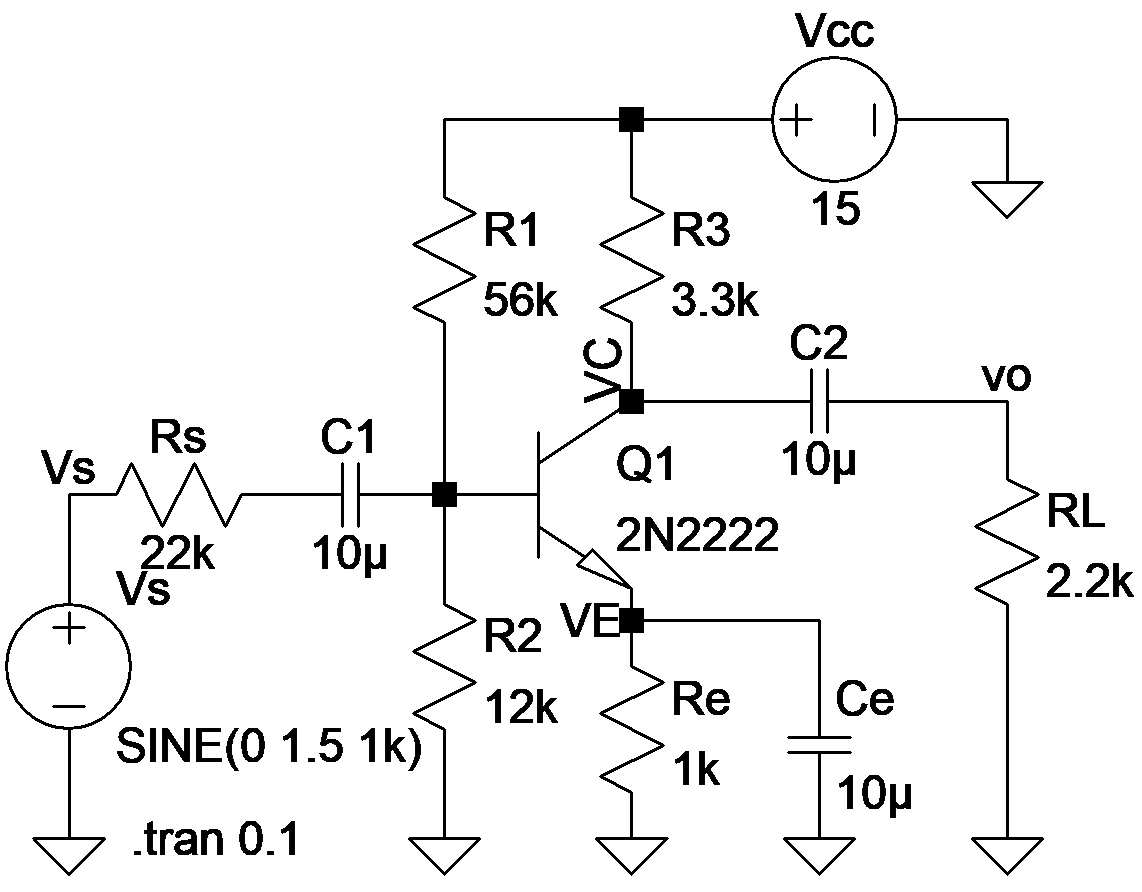
\includegraphics[width=1\linewidth]{e_q3.png}
    
    \small \textit{Circuit 3}
\end{figure}
\end{minipage}\hfill\begin{minipage}{0.49\textwidth}
\begin{figure}[H]
    \centering
    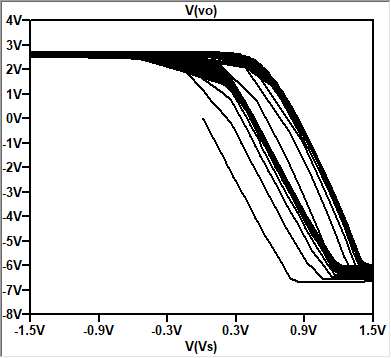
\includegraphics[width=0.9\linewidth]{LTspice_XDvwMEoxIe.png}

    \small \textit{Graph 3}
\end{figure}
\end{minipage}

\newpage

\item For $V_s=0.5V_{pp}$, the amplitude becomes $0.25\text{ V}$. The circuits and the graphs:

\begin{minipage}{0.47\textwidth}
\begin{figure}[H]
    \centering
    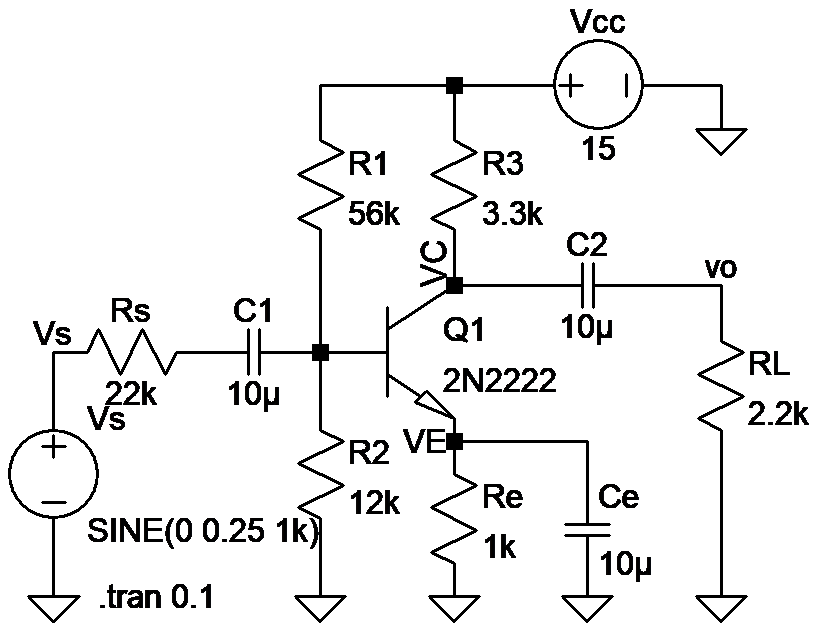
\includegraphics[width=1\linewidth]{e_q4_1.png}
    
    \small \textit{Circuit 4 with the load}
\end{figure}
\end{minipage}\hfill\begin{minipage}{0.49\textwidth}
\begin{figure}[H]
    \centering
    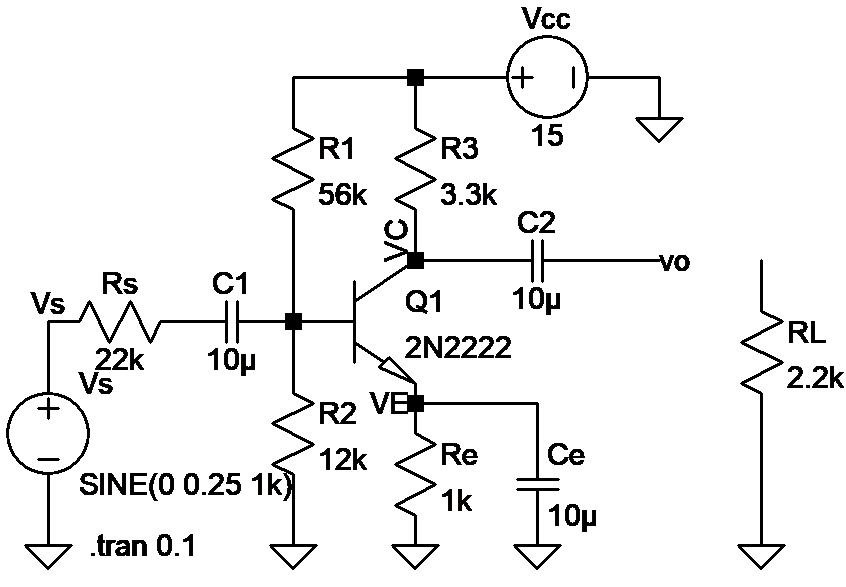
\includegraphics[width=1\linewidth]{e_q4_2.png}

    \small \textit{Circuit 5 without the load}
\end{figure}
\end{minipage}

\begin{minipage}{0.47\textwidth}
\begin{figure}[H]
    \centering
    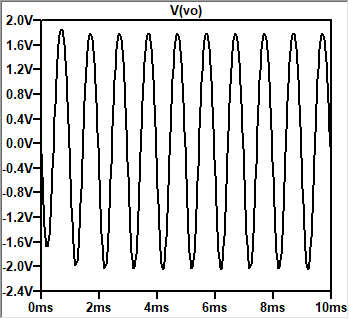
\includegraphics[width=0.92\linewidth]{LTspice_FOCKA3bhwC.png}
    
    \small \textit{Graph 4: Circuit 4 graph}
\end{figure}
\end{minipage}\hfill\begin{minipage}{0.49\textwidth}
\begin{figure}[H]
    \centering
    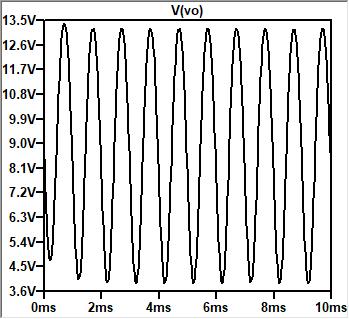
\includegraphics[width=0.9\linewidth]{LTspice_XDd9PN9t43.png}

    \small \textit{Graph 5: Circuit 5 graph}
\end{figure}
\end{minipage}

\end{enumerate}

\end{document}